\section{Experimental Results}

\subsection{Implementation}

\begin{figure}[!ht]
\begin{center}
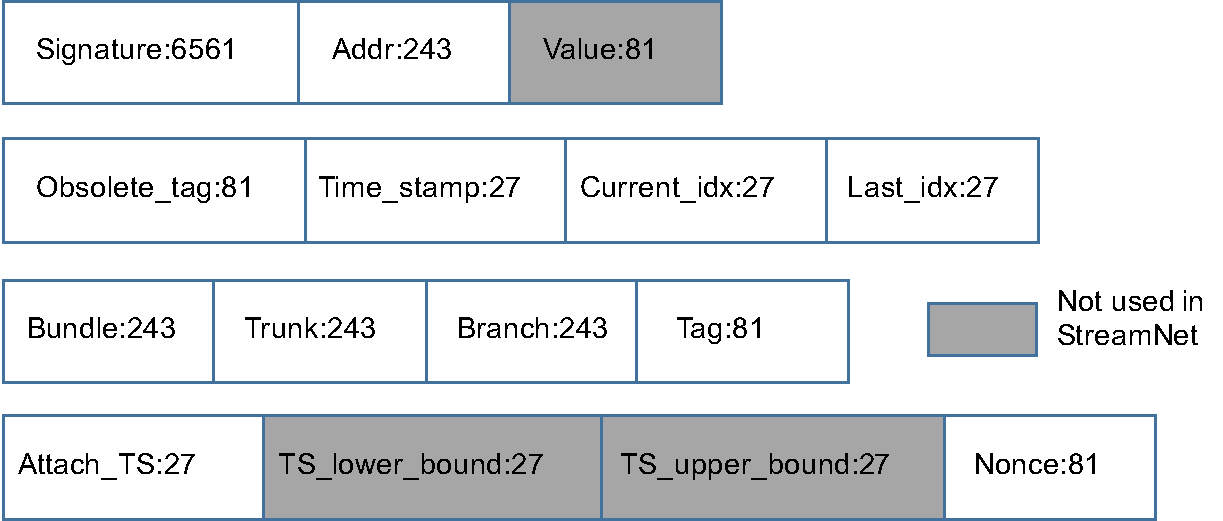
\includegraphics[width=0.45\textwidth]{figures/block_format.pdf}
    \caption{
        Block header format, the main transaction information is stored in the signature part. Addr is sender's address, time stamp is the time the block has been created, current/last index and the bundle are used for storing the bundle information, trunk and branch are the hash address to store the parent and reference location, tag is used for store some tagging information, addtach\_TS is when the block is attached to the StreamNet, nonce is used in POW calculation.
     }
\label{block_header}
\end{center}
\end{figure}

We have implemented the StreamNet based on the IOTA JAVA reference code (IRI) v1.5.5 \cite{IOTACode}.
We forked the code and made our own implementation, the code is freely available at \cite{StreamNet}.
In this paper we use version v0.1.4-streamnet in v0.1-streamnet beta branch.

\begin{itemize}
    \item The features we have adopted from the IRI are: 
    \begin{itemize}
        \item The block header format, as shown in Figure~\ref{block_header}. Some of the data segments are not used in StreamNet which are marked grey.
        \item Gossip network, the network is a bi-directional network in which every node will send and receive data from its peers;
        \item Trasnaction bundle, because of the existence of the bundle hash feature, StreamNet can support both the single transaction for a block and batched transactions as a bundle. 
        \item Sponge hash functions which is claimed to be quantum immune, in our experiment, the POW hardness is set to 8 which is the same as the testnet for IOTA.
    \end{itemize}

    \item The features we have abandoned from the IRI are:
    \begin{itemize}
        \item The iota's transaction logic inlcuding the ledger validation part;
        \item The milestone issued by coordinators, which is a centralized set up. 
    \end{itemize}

    \item The features we have modified based on the IRI is: 
    \begin{itemize}
        \item The tip selection method based on MCMC, since the tip selection on IRI has to find a milestone to start searching, we replace this with a block in the pivotal chain instead.
    \end{itemize}


    \item The features we have added into the StreamNet are: 
    \begin{itemize}
        \item The consensus algorithms, and we have applied the streaming method directly in the algorithms; 
        \item The UTXO logic which is stored in the signature part of the block header, we used the graph data structure to store UTXO as well. 
        \item In IOTA's implementation, the blocks are stored in the RocksDB \cite{RocksDB} as the persistence layer, which makes it inefficient to infer the relationships between blocks and calculate graph features. In our implementation, we introduced an in-memory layer to store the relationships between blocks, such that the tip selection and total ordering algorithm will be accelerated. 
    \end{itemize}
\end{itemize}

\subsection {Environment Set Up}

\begin{figure*}[!ht]
\begin{center}
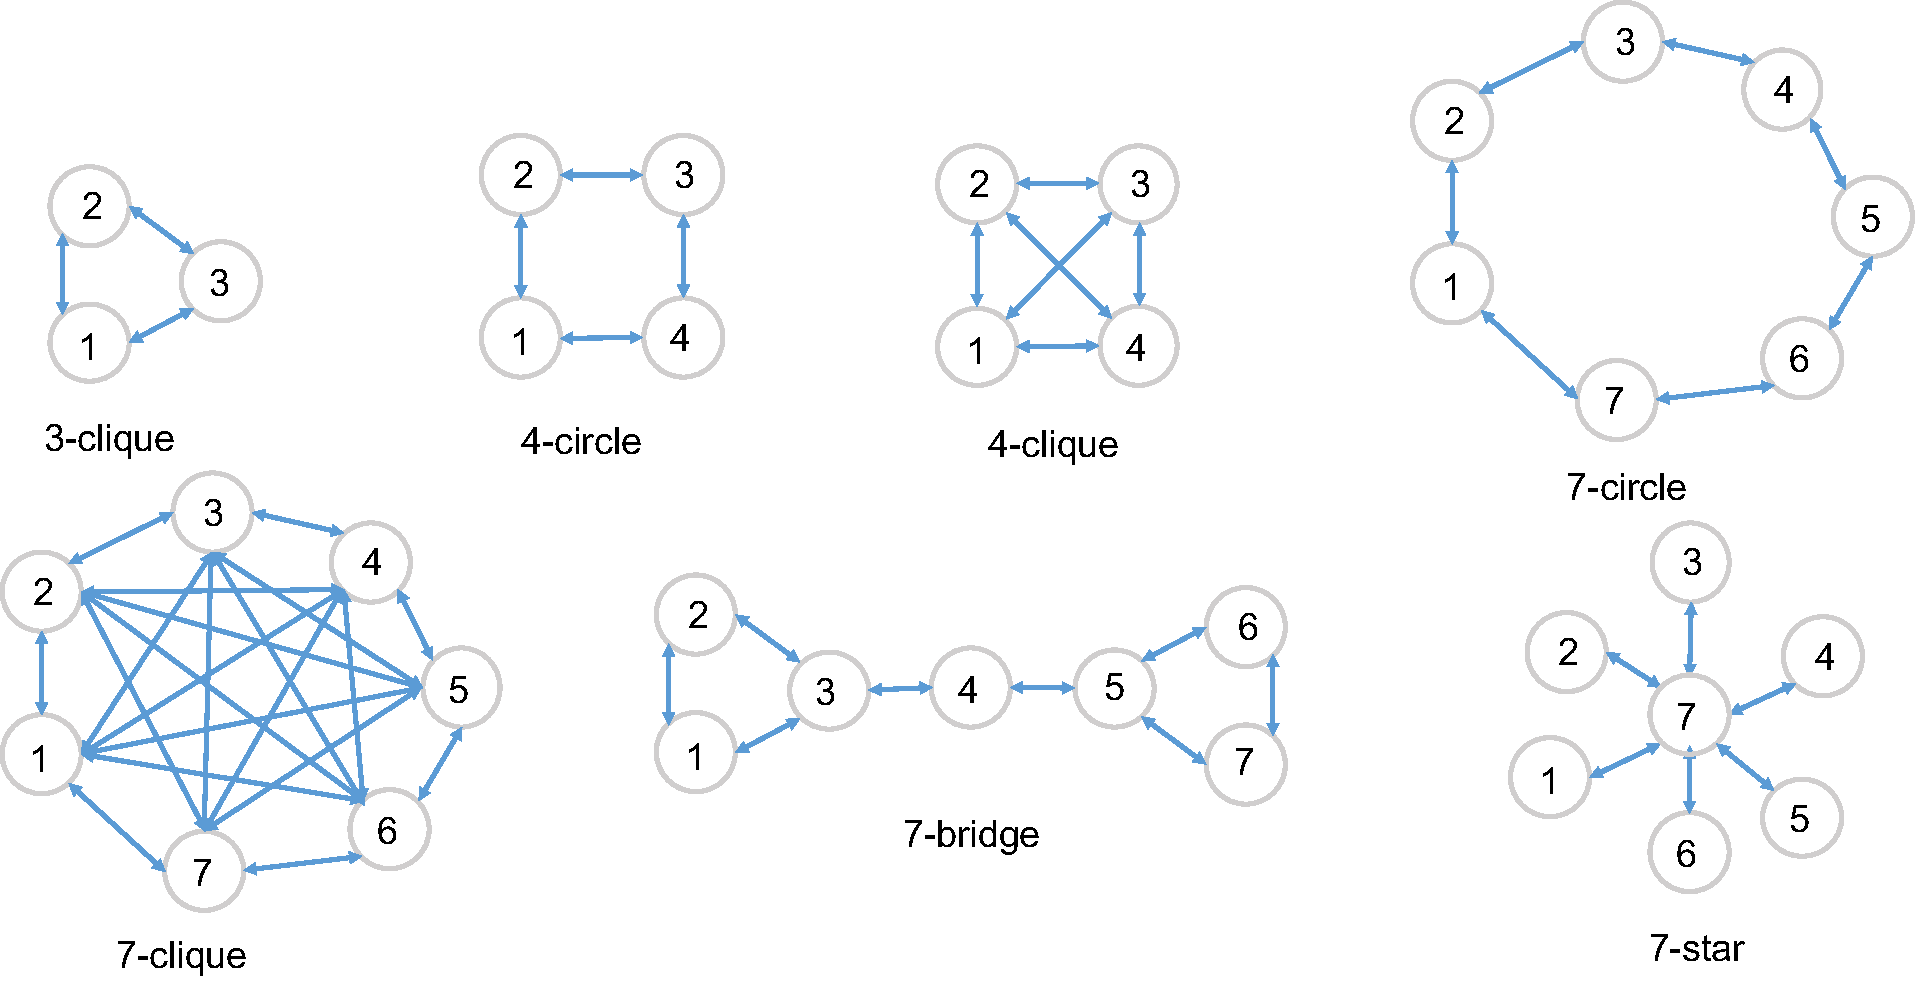
\includegraphics[width=0.75\textwidth]{figures/cluster_set_up.pdf}
    \caption{
        Cluster set up for different network topologies. For 3-cluster configuration only strong computing nodes are involved in the experiment, for 4-cluster and 4-circle, 3 strong and 1 weak computing node are involved in the experiment.
     }
\label{cluster_set_up}
\end{center}
\end{figure*}

We have used the Tencent cloud services with 7 virtual machines, and we have splitted the virtual machines into two different set up with 3 strong nodes and 4 weak nodes. 

\begin{itemize}
    \item For a strong node, it includes a four core Intel(R) Xeon(R) CPU E5-26xx v4, with 15 Gb of memory size and 197Gb of disk size. 
    \item For a weak node, it includes a two core Intel(R) Xeon(R) CPU E5-26xx v4, with 3 Gb of memory size and 118Gb of disk size. 
\end{itemize}
The JAVA version is 1.8, we have deployed our service using docker and the docker version is 18.02.0-ce.   

We have 7 topologies set up of nodes, which are shown in Figure~\ref{cluster_set_up}, these configurations are aiming to test: 
\begin{itemize}
    \item The performance when the cluster connectivity is high (congestion of communications, like 3-clique, 4-clique, 7-clique and 7-star);
    \item The performance when the cluster diameter is high (long hops to pass message, like 4-circle, 7-circle, 7-bridge);
\end{itemize}

As for the data, we have created 1,000 accounts, with the genesis account having 100,000,000,000 tokens in the coinbase block.
We splited the accounts into two groups (each group will have 500 accounts), the first group will participate in the ramp up step, which means the genesis account will distribute the tokens to these accounts.
And for comparison we have issued four set of different size transactions (5000, 10000, 15000 and 20000) respectively.
In the execution step, the first group of accounts will issue transactions to the second group of accounts, which constructs a bipartite spending graph. 
Since there are more transactions than the number of accounts, there will be double spend manners in this step.
The number of threads in this procedure is equal to the number of nodes for each configuration.
Jmeter is utilized as the driver to issue the transactions and Nginx is used to evenly and randomly distribute the requests to different nodes.

\subsection {Results and Discussions}

\subsubsection {Block generateion rate test}
To test the block generation rate, we set each block in StreamNet to have only one transaction.
And the performance on this configuration is as Figure~\ref{single_txn} shows.
To begin with, as the size of the cluster grows, the network as a whole will witness little performance loss on all of the data scales. 
This is because in IOTA implementation, when a node receives data from its peers, it will run a new POW to check the nonce and hash, by the time of this paper is written, 
we do not delve into the detail of whether this could be replaced with a constant time validation process, but the chance is high.
As in the gossip network, a node can not distinguish if the block is generated by itself or if the block is already consumed, it will run redundant checks, this can explain
the reason why as the complexity of the network topology grows, the TPS reduces (In figure we can see that TPS(4-circle)$>$TPS(4\-clique) and TPS(7-star)$>$TPS(4-bridge)$>$TPS(4-circle)$>$TPS(4-clique)).  
We can also observe the performance thrashing in the results, 
this is because for some times, the flood of the blocks will hit the memory limit of the weak nodes, which will cause the out of memory (OOM) error and let the node shut down. 
As the system scale and complexity of the network growing, we will see this performance thrashing issue more often.

In the experiment, we can also see that with the growth of the data, the reduction of the TPS ratio is less than the ratio of the growth of the data (1-2 times as oppsed to 4 times).
Considering the system is dealing the a growing graph instead of a chain, and the complexity analysis in the previous section,
our streaming algorithm shed the light on how to deal with the complexity of the growing DAG.
And if we can find a way to snapshot the DAG in a decentralized way (for instance pushing the genesis ahead), the real stability can be achieved.

\begin{figure}[!ht]
\begin{center}
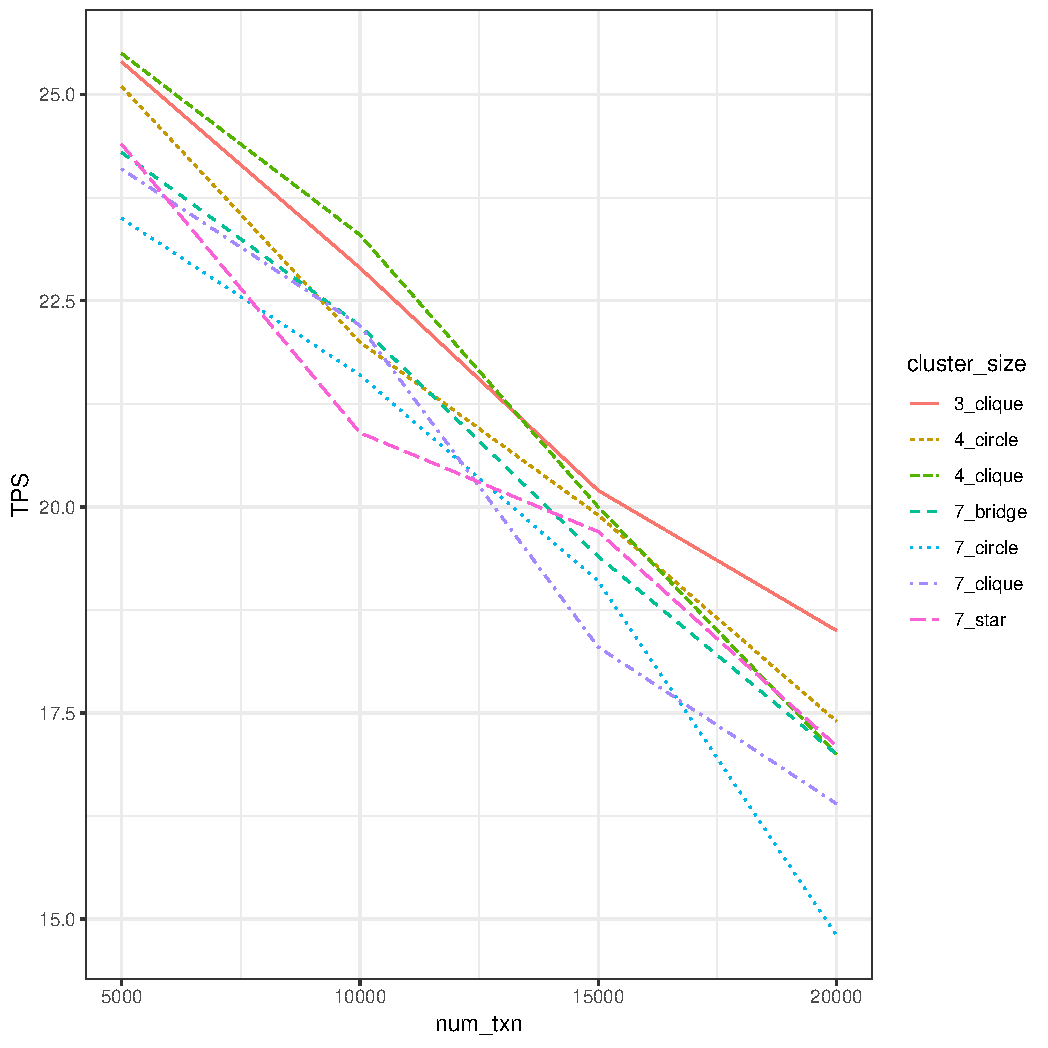
\includegraphics[width=0.45\textwidth]{figures/single_txn.pdf}
    \caption{
        Experimental results for block generation rate.
     }
\label{single_txn}
\end{center}
\end{figure}



\subsubsection {Bundle transaction test}

By default, each block in StreamNet will support bundle transaction. 
Each block will contain 20 transactions.
And the performance on this configuration is as Figure~\ref{multi_txn} shows.
In this experiment, we can see weak scaling effect on every data set, as the performance will grow with the size of the clusters.
This is because of the batching, the total number of the blocks that needs to be calculated is becoming less, and there will be less network message passing.
In addition, the effect of network topology still holds, as the more complex the network structure, the less efficiently it will perform.
One thing to note is that, as the data size grows, the performance degration for the smaller cluster will be more than the larger cluster.
This is because in the small cluster, small number of nodes will process large amount of data, which will soon flood the memories of the neighbor nodes, which will result in a sharp performance down turn.
And in the bundle transaction test, we see much less performance thrashing because there are much less number of blocks passed in the network. 

\begin{figure}[!ht]
\begin{center}
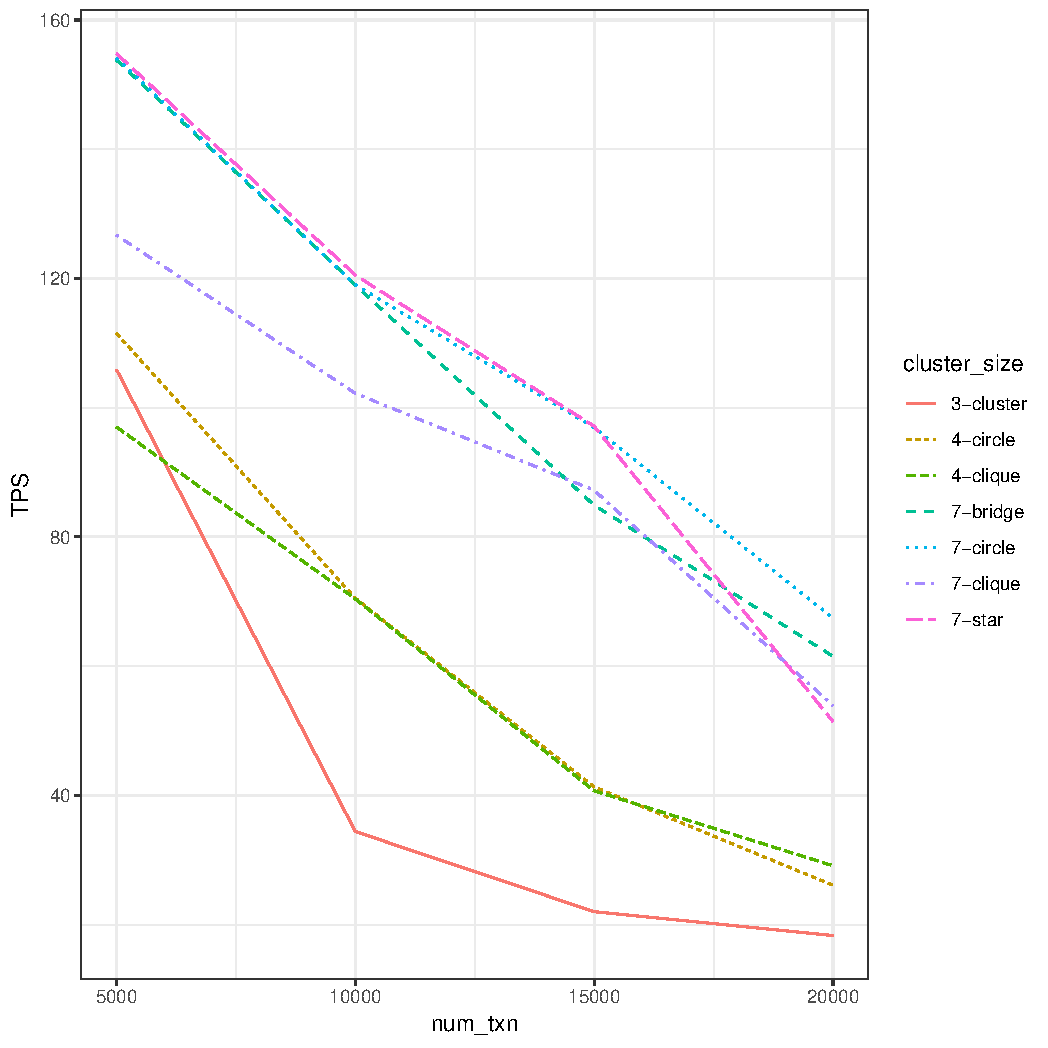
\includegraphics[width=0.45\textwidth]{figures/multi_txn.pdf}
    \caption{
        Experimental results for bundle transaction.
     }
\label{multi_txn}
\end{center}
\end{figure}


